\section{Introduction}
\label{sec:egolog_intro}
\begin{figure}[ht]
  \centering
    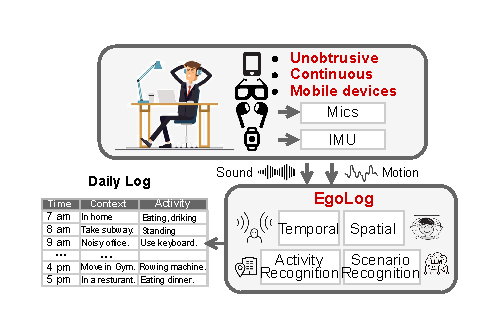
\includegraphics[width=1\linewidth]{chapters/egolog/figs/teaser.pdf}
    \caption{EgoLog uses microphones and an IMU on mobile and head-mounted devices for activity and scenario sensing.}
    \label{fig:egolog_teaser}
    \vspace{-1em}
\end{figure}

% HAR is important
Human activity recognition supports applications in physical and mental health monitoring, personalized healthcare, and daily routine analysis \citep{alam2014gesmart, gedam2021review}.
Smartphones and wearable devices can capture continuous sensor data during daily routines.
For example, motion data from an inertial measurement unit (IMU) can support human activity recognition because it reflects body movement. IMU-based systems have been developed for activities such as walking, standing, sitting, and lying~\citep{smartphonebased_recognition_of_human_activities_and_postural_transitions_341}.
Built-in microphones can also support acoustic scene recognition~\citep{martin2021low}, which provides contextual evidence for human activity.


% the limitation of previous work
However, existing HAR methods on mobile devices are limited to coarse-grained, scenario-constrained detection. For instance, step counting is a common application, but it fails to capture diverse activities such as cycling, swimming, or strength training. Although prior work has extended sensing to vital signs, gait analysis, and exercise recognition, these approaches often focus on isolated tasks rather than continuous daily monitoring.

% our problem/target
This chapter develops a mobile sensing system for ubiquitous devices, including earphones and smart glasses, to support continuous tracking of detailed egocentric human activities. The design models daily life from the user's perspective and moves beyond the recognition of short, isolated activities typically collected in laboratory settings. Fine-grained daily logging differs from conventional activity recognition in two ways:
\begin{enumerate}
    \item Daily life contains long-term activity structure, referred to here as ``scenarios.'' For instance, a user may spend an afternoon at the office while performing many related short-term activities.
    \item Daily life involves continuous interaction with the environment. Consequently, microphones capture sounds from the user, the environment, and other people. These environmental inputs can provide useful context, but they can also introduce noise.
\end{enumerate}


% device and modality
Several types of mobile devices are suitable for this task, including earphones, glasses, smartphones, and smartwatches. This thesis emphasizes head-mounted wearables because they are suitable for day-long use and provide stable egocentric observations, but the core audio--motion sensing design also applies to other mobile form factors. The available sensors can be roughly divided into two categories: visual and non-visual.
Visual sensors, such as cameras, can capture a first-person view rich with information. However, they are less practical for daily logging due to several limitations: 1) a limited field of view (FOV), 2) privacy concerns, and 3) high energy consumption for continuous sensing.
Instead, EgoLog uses non-visual sensors, namely motion and audio sensors. These sensors are widely available on smartphones, glasses, smartwatches, and earphones. As Fig. \ref{fig:egolog_teaser} shows, EgoLog continuously monitors a user's activities from an egocentric perspective and generates a daily log that includes both short-term activities and long-term scenarios.



% mobile devices have been a popular category of wearable devices that equip multiple sensors, such as microphones and IMUs. Being able to capture data from the user's ego view, mobile devices can be a desired platform for sensing detailed user-egocentric activities.
% First, earphone is the most popular wmobile devices with various applications including activity \citep{mollyn2022samosa}, speech \citep{he2023towards, dong2024rehearsse}, pose estimation \citep{duan2025argus}, eye tracking \citep{jiao2024medusa3d}, and vital signs \citep{chen2024exploring}.
% In 2025, there are more than 355 million mobile devices (e.g., earphones) sold, accounting for more than 60\% of wmobile devices worldwide \citep{Idc_2025}.
% Second, earphone is built with rich sensing capability, i.e., a microphone on each ear and an IMU. The sensors can capture stereo audio and motion that reflects egocentric information, such as user-induced speech and activities, and the location of environmental activities.
% Third, mobile devices are ideal for continuous sensing, the location of mobile devices is in the same place without the interference of the user's motion, and there is no blockage like a smartphone when it is placed in the pocket for most of the time.
% Besides, the average American young people use mobile devices more than 400 hours per year \citep{Ferjan_2022}, making it ideal for collecting continuous data.

This task introduces three challenges:
\begin{itemize}
    \item Existing mobile devices HAR models \citep{bhattacharya2022leveraging, gong2023mmg} lack the awareness of scenario information present in the real world. Specifically, user activities are driven by underlying reasons, and their distribution varies depending on the ``scenario.''  For instance, in an ``indoor cooking'' scenario, the ``jogging'' activity is less likely to happen.
    \item HAR models that depend on audio recordings are susceptible to interference due to the lack of spatial understanding. As a result, the audio data may lead to potential errors, which can be harmful for post-processing. For example, when detecting a ``clap'' activity based on sound, a nearby person's action could also trigger the model.
    \item Multi-modal fusion of audio and IMU is challenging and may not outperform a unimodal model \citep{huang2022modality}. Sensor heterogeneity weakens cross-modal alignment, as also observed in MMG-Ego4D \citep{gong2023mmg}. Effective fusion therefore requires models that identify when audio and motion are complementary.
\end{itemize}

To address these challenges, EgoLog uses the following design:
First, EgoLog recognizes long-term scenarios through temporal understanding, as detailed in Sec. \ref{sec:egolog_scenario}. This is achieved using a two-stage model: contrastive learning first projects audio and IMU features into a shared space to identify well-aligned segments as informative key frames; a sequence model then aggregates these key-frame features together with the original unimodal features for scenario recognition.

Second, EgoLog distinguishes user-generated activities from environmental sounds, including sounds produced by other people, through spatial understanding (Sec.~\ref{sec:egolog_localization}). The system formulates this as a sound localization task: near-field sounds are treated as user-centric events, while far-field sounds are treated as ambient background. A motion-aware localization model uses natural human movement and IMU readings to compensate for user motion and reduce spatial ambiguities such as near-far confusion.


Third, EgoLog introduces a multi-modal network for activity recognition that integrates audio, IMU, and scenario information (Sec.~\ref{sec:egolog_har}). Unlike short-term sensor data, the derived scenario captures longer-term behavioral patterns and provides high-level semantic cues for activity recognition.
The network uses dedicated unimodal backbones for feature extraction and a self-attention mechanism to dynamically fuse multimodal inputs, with scenario information encoded as a dense representation through a text encoder.

Finally, in Section \ref{sec:egolog_llm}, EgoLog introduces an edge-cloud framework assisted by a Large Language Model (LLM) for scenario recognition. The framework converts multi-modal data, including audio, IMU signals, sound localization outputs, and local scenario predictions, into contextual information for the LLM.
When the local model's prediction confidence is low, the edge device queries the cloud-based LLM. The refined scenario output is then used to update the local model over time.


We implemented and evaluated EgoLog on three large-scale public datasets, including Ego4D~\citep{grauman2022ego4d}, and a self-collected dataset covering multiple form factors, 10 participants, and 12 activities.
EgoLog improves activity recognition by 12\% and scenario recognition by 15\% over strong multi-modal baselines such as ImageBind~\citep{girdhar2023imagebind}, while keeping computation cost low.
The main contributions of this chapter are as follows:


\begin{itemize}
    \item
    EgoLog introduces an audio--IMU fusion method based on temporal and spatial understanding. It extracts scenario-level features through contrastive learning, aggregates them across short-term windows for scenario recognition, and integrates motion information with sound source localization for movement compensation.

    \item
    EgoLog develops an HAR method that takes both scenario context and raw sensor data as input. It uses scenario information to distinguish similar activities and uses sound-source estimates with audio--IMU correlation to separate user-generated sounds from background sounds.

    \item
    EgoLog introduces an LLM-assisted scenario recognition paradigm. Processed sensor data is fed into an LLM for high-level reasoning, and the LLM output is transferred back to the local device for on-device inference.

    \item
    EgoLog is evaluated on public datasets and a self-collected dataset, with an additional user study on the usefulness of generated daily summaries. The evaluation shows improvements of up to 15\% over the strongest baselines.
\end{itemize}
